\documentclass[11pt, a4paper, copyright]{google}

\usepackage{tikz}
\usepackage{multicol}
\usetikzlibrary{positioning,arrows.meta,shapes.geometric,fit,backgrounds,calc,decorations.pathreplacing}

\usepackage[authoryear, sort&compress, round]{natbib}
\bibliographystyle{abbrvnat}

\makeatletter
\renewcommand{\absfont}{\normalfont\linespread{1.2}\fontsize{11}{12}\selectfont}

% Princeton-themed abstract box
\definecolor{princetonorange}{HTML}{E77500}
\definecolor{absboxbg}{HTML}{FFF8F0}
\definecolor{absboxframe}{HTML}{E77500}
\renewcommand{\abscontent}{%
  \noindent
  \begin{tcolorbox}[
    colback=absboxbg,
    colframe=absboxframe,
    boxrule=0.8pt,
    arc=3pt,
    left=10pt, right=10pt, top=8pt, bottom=8pt,
    fonttitle=\bfseries\large,
    title=Abstract,
    coltitle=white,
    attach boxed title to top left={yshift=-\tcboxedtitleheight/2, xshift=12pt},
    boxed title style={colback=princetonorange, colframe=princetonorange, boxrule=0pt, arc=2pt, left=6pt, right=6pt, top=2pt, bottom=2pt}
  ]
  {\absfont \theabstract}
  \@ifundefined{@keywords}{}{%
    \vskip0.8em \noindent \keywordsfont Keywords: \@keywords}
  \end{tcolorbox}%
}
\makeatother
\definecolor{linkblue}{RGB}{0,0,139}
\definecolor{navy}{RGB}{0,0,128}
\definecolor{royalblue}{RGB}{65,105,225}
\definecolor{steelblue}{RGB}{70,130,180}
\definecolor{dodgerblue}{RGB}{30,144,255}
\definecolor{mediumblue}{RGB}{0,0,205}
\definecolor{darkslateblue}{RGB}{72,61,139}
\usepackage[colorlinks = true,
            linkcolor = linkblue,
            urlcolor  = royalblue,
            citecolor = brown,
            anchorcolor = blue]{hyperref}

\usepackage[misc]{ifsym}
\usepackage{minitoc}
\usepackage{cleveref}
\usepackage{subcaption}
\usepackage{booktabs}
\usepackage{amsmath}
\usepackage{mathtools}
\usepackage{amssymb}
\usepackage{graphicx}
\usepackage{algorithmic}
\usepackage{algorithm}
\usepackage{tcolorbox}
\usepackage{verbatim}
\usepackage{makecell}
\usepackage{array}
\usepackage{multirow}
\usepackage{xurl}
\usepackage{amsthm}
\usepackage{adjustbox}
\usepackage{caption}
\usepackage{xcolor}
\usepackage{wrapfig}
\usepackage{pifont}
\usepackage{enumitem}
\usepackage[titles]{tocloft}
\setlength{\cftbeforesecskip}{5pt}
\setlength{\cftbeforesubsecskip}{2pt}
\setlength{\cftbeforesubsubsecskip}{1pt}
% Princeton-themed TOC colors
\definecolor{tocsubsec}{HTML}{444444}
\definecolor{tocsubsubsec}{HTML}{666666}
\renewcommand{\cftsecfont}{\bfseries\color{princetonorange}}
\renewcommand{\cftsecpagefont}{\bfseries\color{princetonorange}}
\renewcommand{\cftsubsecfont}{\color{tocsubsec}}
\renewcommand{\cftsubsecpagefont}{\color{tocsubsec}}
\renewcommand{\cftsubsubsecfont}{\small\color{tocsubsubsec}}
\renewcommand{\cftsubsubsecpagefont}{\small\color{tocsubsubsec}}
\usepackage{soul}

\usepackage{listings}
\tcbuselibrary{listings,skins,breakable}

% \lstdefinestyle{prompt}{
%   basicstyle=\ttfamily\small,
%   breaklines=true,
%   breakatwhitespace=true,   % 避免句号/标点被单独断到下一行
%   columns=fullflexible,
%   keepspaces=true,
%   showstringspaces=false
% }
\lstdefinestyle{prompt}{
  basicstyle=\ttfamily\footnotesize,
  breaklines=true,
  breakatwhitespace=true,
  columns=fullflexible,
  keepspaces=true,
  showstringspaces=false,
  postbreak=\mbox{\textcolor{gray}{$\hookrightarrow$}\space}
}

\newtheorem{corollary}{Corollary}
\newtheorem{remark}{Remark}
\newtheorem{proposition}{Proposition}
\newtheorem{theorem}{Theorem}
\newtheorem{lemma}{Lemma}

\newcommand{\method}{OpenClaw-RL}
\newcommand{\methodshort}{OpenClaw-RL}
\newcommand{\ie}{\textit{i.e.}}
\newcommand{\eg}{\textit{e.g.}}
\newcommand{\etc}{\textit{etc.}}
\newcommand{\wrt}{w.r.t.}
\newcommand{\R}{\mathbb{R}}
\newcommand{\E}{\mathbb{E}}
\newcommand{\KL}{\mathrm{KL}}
\newcommand{\cmark}{\ding{51}}
\newcommand{\xmark}{\ding{55}}

\newcommand{\TODO}[1]{\colorbox{yellow!70}{\textbf{[TODO: #1]}}}
\newcommand{\RESULT}[1]{\colorbox{orange!50}{\textbf{#1}}}

\definecolor{accent1}{HTML}{2E6DA4}
\definecolor{accent2}{HTML}{D9534F}
\definecolor{accent3}{HTML}{5CB85C}
\definecolor{lightblue}{RGB}{173,216,230}
\definecolor{lightorange}{RGB}{255,213,170}
\definecolor{lightgreen}{RGB}{176,226,176}
\definecolor{lightyellow}{RGB}{255,255,204}
\definecolor{lightgray}{RGB}{220,220,220}
\definecolor{lightpurple}{RGB}{221,160,221}
\definecolor{lightred}{RGB}{255,182,193}
\definecolor{gray60}{gray}{0.6}
\definecolor{accent4}{HTML}{9B59B6}

\uselogo{}

% Inject code link between authors and abstract box
\makeatletter
\renewcommand{\abscontent}{%
  \begin{center}
  {\fontsize{11pt}{13pt}\selectfont \raisebox{-0.06em}{
\includegraphics[height=1em]{assets/git.png}}\;\href{https://github.com/Gen-Verse/OpenClaw-RL}{\texttt{https://github.com/Gen-Verse/OpenClaw-RL}}}
  \end{center}
  \vskip0.8em
  \noindent
  \parbox{\dimexpr\linewidth}{\absfont \theabstract}%
  \@ifundefined{@keywords}{}{%
    \vskip1em \noindent \keywordsfont Keywords: \@keywords}%
}
% Center title and author list
\renewcommand{\maketitle}{\bgroup\setlength{\parindent}{0pt}
  \begin{adjustwidth}{0pt}{24pt}
    \begin{center}
      {\titlefont \@title\par}%
      \vskip11pt
      {\@author\par}%
      \vskip20pt%
    \end{center}
  \end{adjustwidth}
  \egroup
  {\abscontent}%
  \thispagestyle{firststyle}
}
\makeatother

% Only override right header: OpenClaw logo replaces date
\AtBeginDocument{%
  \fancypagestyle{firststyle}{%
    \fancyhead[L]{
\includegraphics[height=27pt]{assets/logo}}%
    \fancyhead[R]{
\includegraphics[height=27pt]{assets/openclaw-logo}}%
    \fancyhead[C]{}%
    \fancyfoot[L]{%
  \footerfont
  $^{*}$Equal contribution;\quad $^{\dagger}$Corresponding authors;\quad
  \ifdefined\correspondingauthor
    \if\relax\the\correspondingauthor\relax
    \else
      {\itshape \the\correspondingauthor}%
    \fi
  \fi
  \\
  \ifthenelse{\boolean{copyright}}{\copyrightext}{}%
}%
    \fancyfoot[R]{\footerfont\bfseries\relax}%
    \fancyfoot[C]{\footerfont\bfseries\relax}%
  }%
}

% ============================================================
% Title / Authors
% ============================================================
\title{OpenClaw-RL: Train Any Agent Simply by Talking}

\correspondingauthor{Main contact: yangling0818@163.com}

% Suppress authblk superscript marks and fix comma spacing
 \makeatletter
% \renewcommand\AB@authnote[1]{}
 \renewcommand\AB@affilnote[1]{}
 \makeatother
 \renewcommand\Authands{, }

\author[*]{Yinjie Wang}
\author[*]{Xuyang Chen}
\author[*]{Xiaolong Jin}
\author[$\dagger$]{Mengdi Wang}
\author[$\dagger$]{Ling Yang}

\affil{}

\begin{abstract}
Every agent interaction generates a \textbf{next-state signal}, namely the user reply, tool output, terminal or GUI state change that follows each action, yet no existing agentic RL system recovers it as a live, online learning source.
We present \textbf{OpenClaw-RL}, a framework built on a simple observation: next-state signals are universal, and policy can learn from all of them simultaneously.
Personal conversations, terminal executions, GUI interactions, SWE tasks, and tool-call traces are not separate training problems. They are all interactions that can be used to train the same policy in the same loop.
Next-state signals encode two forms of information: \textit{evaluative signals}, which indicate how well the action performed and are extracted as scalar rewards via a PRM judge; and \textit{directive signals}, which indicate how the action should have been different and are recovered through \textbf{Hindsight-Guided On-Policy Distillation (OPD)}. We extract textual hints from the next state, construct an enhanced teacher context, and provide token-level directional advantage supervision that is richer than any scalar reward.
Due to the asynchronous design, the model serves live requests, the PRM judges ongoing interactions, and the trainer updates the policy at the same time, with zero coordination overhead between them.
Applied to \textbf{personal agents}, OpenClaw-RL enables an agent to improve simply by being used, recovering conversational signals from user re-queries, corrections, and explicit feedback.
Applied to \textbf{general agents}, the same infrastructure supports scalable RL across terminal, GUI, SWE, and tool-call settings, where we additionally demonstrate the utility of process rewards.
\end{abstract}





\begin{document}

\maketitle

\begin{figure}[h]
  \centering
  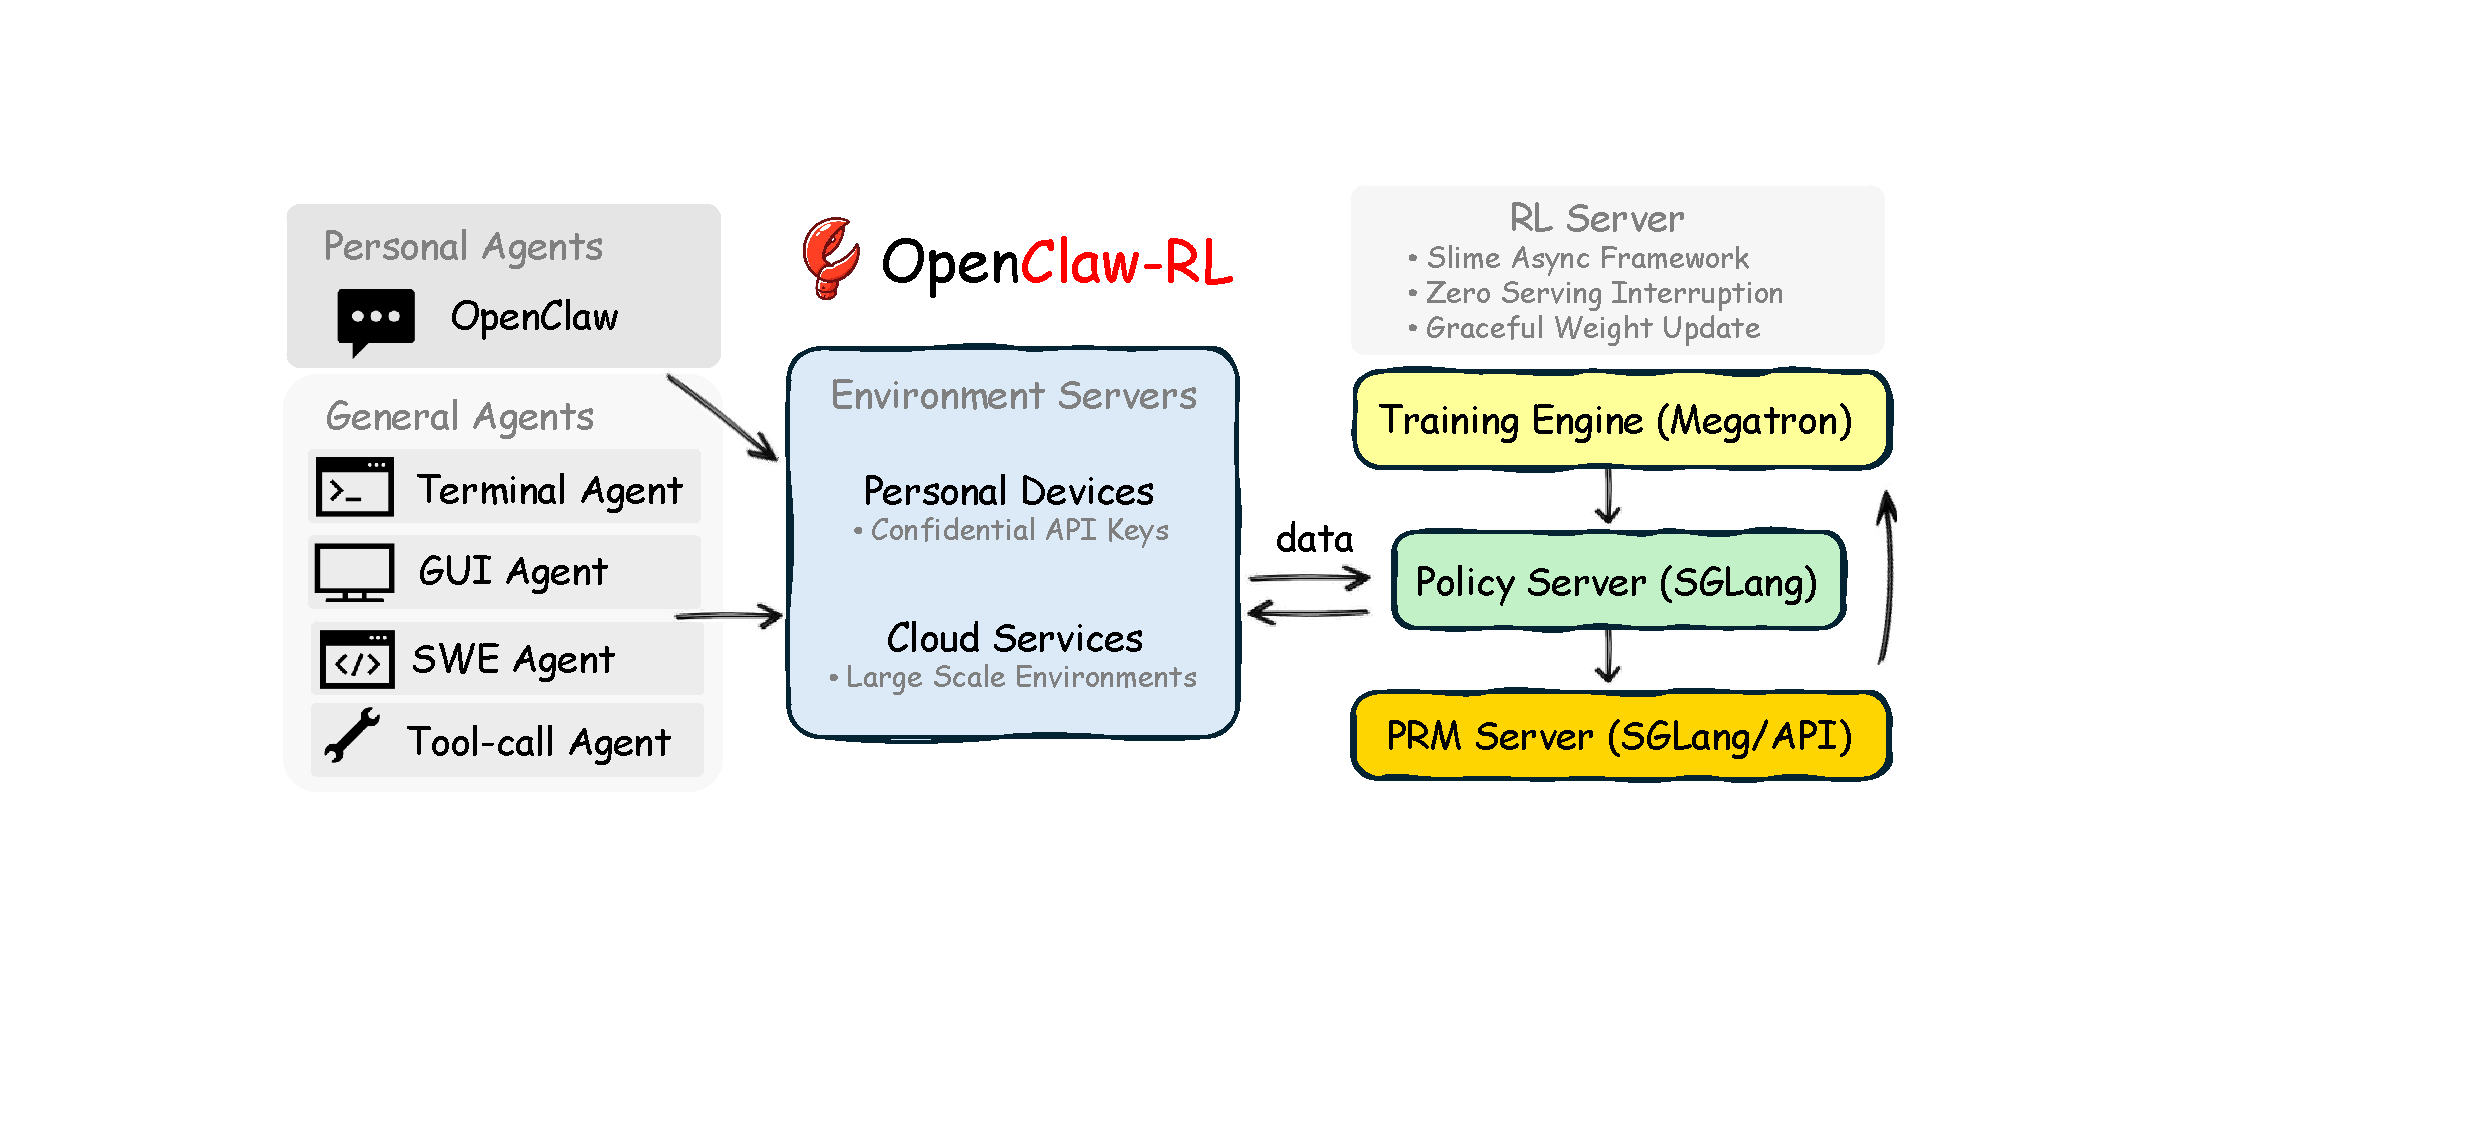
\includegraphics[width=\linewidth]{assets/framework.pdf}
  \caption{
    \textbf{OpenClaw-RL infrastructure overview.}
    Interaction streams come from two agent types: \textit{Personal Agents} (conversational, single-user), hosted on personal devices, and \textit{General Agents} (terminal, GUI, SWE, and tool-call agents), hosted on cloud services.
The collected samples flow into our RL server built on the asynchronous \textbf{slime} framework, which consists of four \textit{decoupled components}: (1)~the environment server, (2)~\textbf{PRM\,/\,Judge} for reward computation, (3)~\textbf{Megatron} for policy training, and (4)~\textbf{SGLang} for policy serving. These components support graceful weight updates and enable training with \textbf{any} agentic framework.
The environment for personal agents is simply the users' personal devices, which connect to the RL server over HTTP with confidential API keys. The environments for general agents are hosted on cloud services to enable scalable parallelization.
  }
  \label{fig:framework}
\end{figure}





\newpage
\vspace{0.5em}
{
  \hypersetup{linkcolor=black}
  \setlength{\parskip}{0pt}
  \renewcommand{\contentsname}{\normalfont\large\bfseries Contents}
  \setcounter{tocdepth}{3}
  \begingroup
    \small
    \tableofcontents
  \endgroup
}
% \vspace{0.5em}
% \hrule
% \vspace{1em}




\newpage

% ============================================================
% 1. Introduction
% ============================================================






\section{Introduction}
\label{sec:intro}

Every deployed AI agent is already collecting the data it needs to improve and discarding it.
After each action $a_t$, the agent receives a \textbf{next-state signal} $s_{t+1}$: a user reply, a tool execution result, a GUI state transition, or a test verdict.
Existing systems treat this purely as context for the next action \citep{sheng2025hybridflow, slime_github, mei2025real, fu2025areal, wang2025reinforcement}. We argue that next-state signals encode something more valuable: an implicit evaluation of $a_t$, including how well it performed and, often, how it should have been different.
Critically, this signal arises for free across every interaction type, including personal conversations, terminal environments, GUI environments, SWE tasks, and tool-call environments, yet no existing agentic RL system recovers them as a live, online learning source 
We identify two distinct and recoverable forms of waste.

\paragraph{Waste 1 --- Evaluative signals.}
The next-state signal implicitly scores the preceding action: a user re-query signals dissatisfaction, a passing test signals success, and an error trace signals failure.
This forms a natural process reward and requires no separate annotation pipeline, yet PRMs have been studied almost exclusively in mathematical reasoning with verifiable ground truth~\citep{lightman2023let, wang2024math, cui2025process}.
In personal agents, it captures user satisfaction turn by turn.
In general agents, it provides the dense per-step credit assignment that long-horizon tasks require~\citep{wang2026rlanything}.
Existing systems either ignore this signal or exploit it only in offline, pre-collected form, relying on fixed datasets or terminal outcome rewards.

\paragraph{Waste 2 --- Directive signals.}
Beyond scoring, next-state signals often carry \textit{directive} information: a user who says ``you should have checked the file first'' specifies not only that the response was wrong, but also how it should change at the token level.
Likewise, a detailed SWE error trace often implies a concrete correction direction.
Current RLVR methods use scalar rewards and thus cannot convert such information into a directional policy gradient~\citep{shao2024deepseekmath, guo2025deepseek, hu2025open, yu2025dapo}, while distillation methods~\citep{shenfeld2026self, hubotter2026reinforcement} rely on pre-curated feedback-response pairs rather than live signals.
Hindsight relabeling~\citep{hubotter2026reinforcement, zhang2023wisdom} and context-enriched distillation~\citep{yang2024buffer,yang2025supercorrect} show that adding structured correction information to the context can substantially improve outputs, but these methods all operate on fixed datasets.
In concurrent work, \citet{kleinebuening2026aligning} improves online policy by directly prompting with next-state information, but the corrective hints remain implicit.




\paragraph{OpenClaw-RL.}
We present \method{}, a unified framework that recovers both forms of next-state signal waste for \textbf{personal agents} and \textbf{general-purpose agents} across diverse settings, including personal conversations with OpenClaw \citep{openclaw2026}, terminal, GUI, SWE, and tool-call environments.
\method{} is a \textbf{fully decoupled asynchronous architecture} built on slime \citep{slime_github}, where policy serving, rollout collection, PRM judging, and policy training run as four independent loops with no blocking dependencies.
In the personal-agent setting, the model can be optimized automatically through normal usage.
This extends existing RL infrastructure, which typically assumes batch data collection rather than continuous learning from live deployment.
We provide two optimization options.
First, binary RL uses a PRM to recover conversations as scalar process rewards.
Second, our \textbf{Hindsight-Guided On-Policy Distillation (OPD)} extracts textual hints from the next state, constructs an enhanced teacher context, and distills token-level directional supervision back into the student, providing training signals unavailable from scalar rewards alone.
\begin{figure}[h]
  \centering
  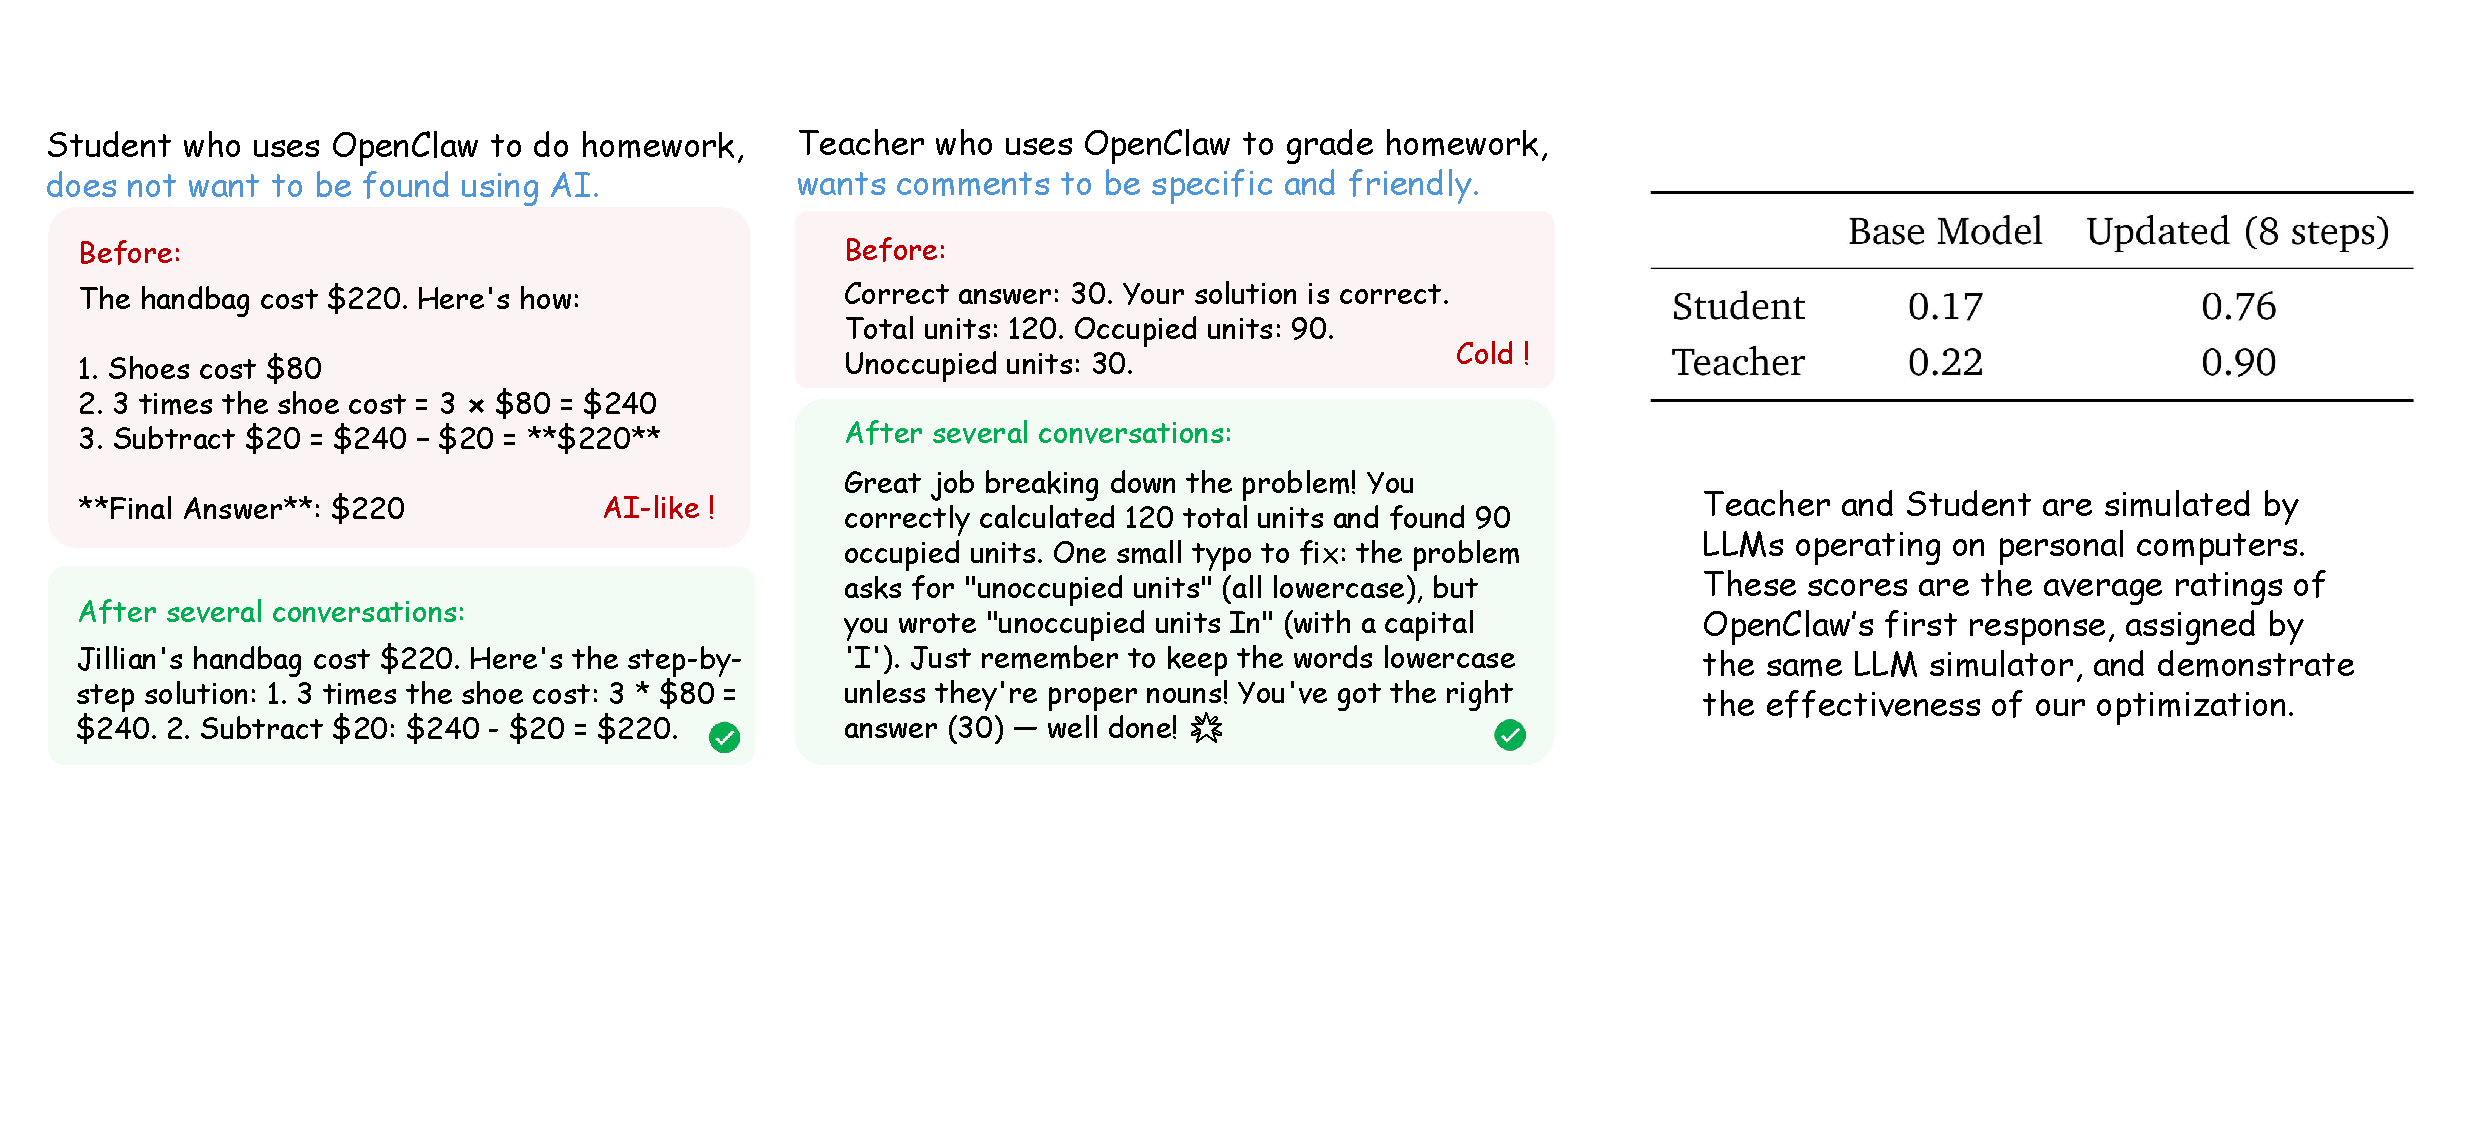
\includegraphics[width=\linewidth]{assets/start1.pdf}
  \vspace{-6mm}
  \caption{Optimize your OpenClaw simply by using it. We provide a simulation result here.}
  \label{fig:start1}
\end{figure}
In simulation experiments, we find that combining the two methods with a weighted loss yields significant gains.
Our framework also extends to RL training for general agents, including terminal, GUI, SWE, and tool-call settings. We integrate PRM judging with verifiable outcomes to provide supervision that is both dense and reliable \citep{wang2026rlanything, zou2025reasonfluxprm}. We further enhance the scalability of this framework by allowing environments to be hosted at scale on cloud services.




\paragraph{Contributions.}
\begin{itemize}[leftmargin=*,itemsep=1pt]
    \item \textbf{Next-state signal as a live, online learning source.} We identify that next-state signals, whether user replies, execution results, test verdicts, or GUI transitions, encode both evaluative and directive information about the preceding action. We recover these signals as a live, online training source across heterogeneous interaction types.

    \item \textbf{OpenClaw-RL Infrastructure.} The first system to unify \textit{multiple concurrent interaction streams}, including personal conversations, terminal, GUI, SWE, and tool-call agentic settings. It is designed for zero interruption to serving, with session-aware multi-turn tracking, graceful weight updates, flexible PRM support, and large-scale environment parallelization.

    \item \textbf{Two complementary next-state signal recovery methods.} Binary RL via PRM converts evaluative next-state signals into dense scalar process rewards, while our Hindsight-Guided OPD converts directive signals into token-level advantage supervision by extracting textual hints from the next state and constructing an enhanced teacher context, where rich textual feedback provides directional guidance for improvement.

    \item \textbf{Empirical validation across personal and general agents.} We validate \method{} in experiments on both personal agent personalization and agentic RL across terminal, GUI, SWE, and tool-call settings. We provide evidence that binary RL and Hindsight-Guided OPD are complementary, and that their combination yields significant gains for personal agents. We also validate the effectiveness of integrating process and outcome rewards in the general-agent RL setting.
\end{itemize}


% ============================================================
% 2. Preliminaries
% ============================================================
\section{Problem Setting}
\label{sec:setting}

\method{} operates on a policy $\pi_\theta$ that simultaneously receives \textbf{multiple interaction streams}, decouples them from the inference pipeline, and is therefore flexible enough for a wide range of agentic settings, including personal agent conversations, terminal executions, GUI interactions, SWE tasks, and tool-call traces. We formalize each interaction stream as a MDP $(\mathcal{S}, \mathcal{A}, \mathcal{T}, r)$:
\begin{itemize}[leftmargin=*,itemsep=2pt]
    \item \textbf{State} $s_t \in \mathcal{S}$: the full conversational or environmental context up to turn $t$.
    \item \textbf{Action} $a_t \in \mathcal{A}$: the agent's response, a sequence of tokens generated by $\pi_\theta$.
    \item \textbf{Transition} $\mathcal{T}(s_{t+1} \mid s_t, a_t)$: deterministic given the environment; $s_{t+1}$ is the user reply, execution result, or tool output that follows $a_t$.
    \item \textbf{Reward} $r(a_t, s_{t+1})$: inferred from the next-state signal via a PRM judge.
\end{itemize}

In standard RLVR, the outcome $o$ serves as the reward for the entire trajectory. However, the process reward $r(a_t, s_{t+1})$, which depends on the next state $s_{t+1}$, contains much richer signals. In particular, when next state contains explicit directive information about how the action should have been different, on-policy distillation enables directional improvement \citep{agarwal2024policy, hubotter2026reinforcement} by converting such directional next-state signals into token-level teacher supervision.





% ============================================================
% 3. Infrastructure
% ============================================================
\section{OpenClaw-RL Infrastructure: Unified System for Personal and General Agents}
\label{sec:infra}

\textit{We unify automatic optimization of personal OpenClaw agents and large scale agentic RL for general agents, including terminal, GUI, SWE, and tool-call settings, within a single framework.}



\subsection{Asynchronous Pipeline with Four Decoupled Components}
\label{sec:infra_overview}

The core architectural principle of \method{} is \textbf{full decoupling}: policy serving, environment hosting, PRM judging, and policy training run as four completely independent asynchronous loops with no blocking dependencies between them (Figure~\ref{fig:framework}).

\begin{center}
\texttt{Policy Serving $\;\rightarrow\;$ environment $\;\rightarrow\;$ Reward Judging $\;\rightarrow\;$ Policy Training}\\
\texttt{(SGLang)\;\;\;\;\;\;\; (Http / API)\;\;\;\;\;\; (SGLang / API)\;\;\;\;\;\;\; (Megatron)}
\end{center}

The model serves the next user request while the PRM judges the previous response and the trainer applies gradient updates; none waits for the others.
This is what makes continuous training from live, heterogeneous interaction streams practical: no stream needs to be paused or batched to accommodate another component's schedule.




For personal agents, the model is connected through a confidential API for private and secure deployment, requires no modification to the personal-agent framework, and is updated gracefully without interrupting inference. For large-scale training of general agents, this asynchronous design allows each components to proceed without being blocked, thereby mitigating the long-tail problem caused by long-horizon rollout durations.



\subsection{Session-Aware Environment Server for Personal Agents}
\label{sec:infra_turns}

The environment for a personal agent is the user's device, which connects to our RL server through a confidential API. Each API request is classified into one of two types:
\begin{itemize}[leftmargin=*, itemsep=2pt]
    \item \textbf{Main-line turn}: the agent's primary response and tool execution results, which form trainable samples.
    \item \textbf{Side turn}: auxiliary queries, memory organization, and environment transitions, which are forwarded but do not produce training data.
\end{itemize}
This classification allows the RL framework to precisely identify which turns belong to which sessions, enabling targeted training. Currently, we train only on main-line turns. The message of each new main-line request contains the reaction to the previous turn, whether a user's reply or an environment's execution result.
This becomes the next-state signal $s_{t+1}$ for the previous turn's reward computation.




\subsection{Scalability: From Single-User Personalization to Large-Scale Agent Deployment}
\label{sec:infra_scale}

\method{} is designed to operate across the full spectrum from single-user personal agent to large-scale multi-environment general agent deployment.
For personal agents, the environment is a single user's device and the interaction stream is sparse, session-based, and highly personalized.
Built on slime \citep{slime_github}, \method{} inherits a scalable training infrastructure for general agents, and we further support cloud-hosted environments across diverse agent settings (Section~\ref{sec:infra_parallel}). Hundreds of parallel environments hosted on cloud services produce a dense stream of structured execution signals, enabling scalable RL training.





\subsection{Support for Multiple Real World Scenarios}
\label{sec:infra_parallel}


\method{} supports a broad set of general-agent scenarios that cover the most common real-world deployment settings in our open-source implementation (Table~\ref{tab:settings}).
Terminal agents are a core component of computer-use systems: they are efficient, cheap to scale, and naturally aligned with the text-based interface of LLMs \citep{claudecode2026, codexcli2026, seta}.
GUI agents cover capabilities that terminal agents cannot access directly, such as visual interfaces and pointer-based interactions, making them necessary for more general computer-use tasks \citep{wang2025ui, qin2025ui, wang2025opencua, xue2026evocua}.
SWE agents represent a particularly important class of coding agents, where the environment provides rich executable feedback through tests, diffs, and static analysis \citep{cao2026qwen3}.
Tool-call agents are also critical, since external tools improve both reasoning capability and factual accuracy \citep{feng2025retool}.



\begin{table}[h]
\centering
\small
\caption{Supported agent settings and their environment characteristics.}
\label{tab:settings}
\begin{tabular}{@{}llll@{}}
\toprule
\textbf{Setting} & \textbf{Environment} & \textbf{Next-state signal} & \textbf{Horizon} \\
\midrule
OpenClaw & Personal devices & user response / tool-call results & Long \\
Terminal & Shell execution sandbox & stdout/stderr, exit code & Long \\
GUI & Screen state + accessibility tree & Visual state diff, task progress & Long \\
SWE & Code repository + test suite & Test verdicts, diff, lint output & Long \\
Tool-call & API/function execution & Return values, error traces & Medium \\
\bottomrule
\end{tabular}
\end{table}





\subsection{Non-Blocking Record and Observability}
\label{sec:infra_record}

All interactions and reward evaluations are logged to JSONL in real time: full message history, prompt/response text, tool calls, next-state content, per-vote PRM scores, selected hints (OPD), and accept/reject decisions.
Logging is non-blocking, writes are fire-and-forget on a background thread, adding no latency to the serving or PRM paths.
Record files are purged at each weight update boundary, ensuring logs always correspond to a single policy version.


% ============================================================
% 4. RL Methods
% ============================================================


\begin{figure}[t]
  \centering
  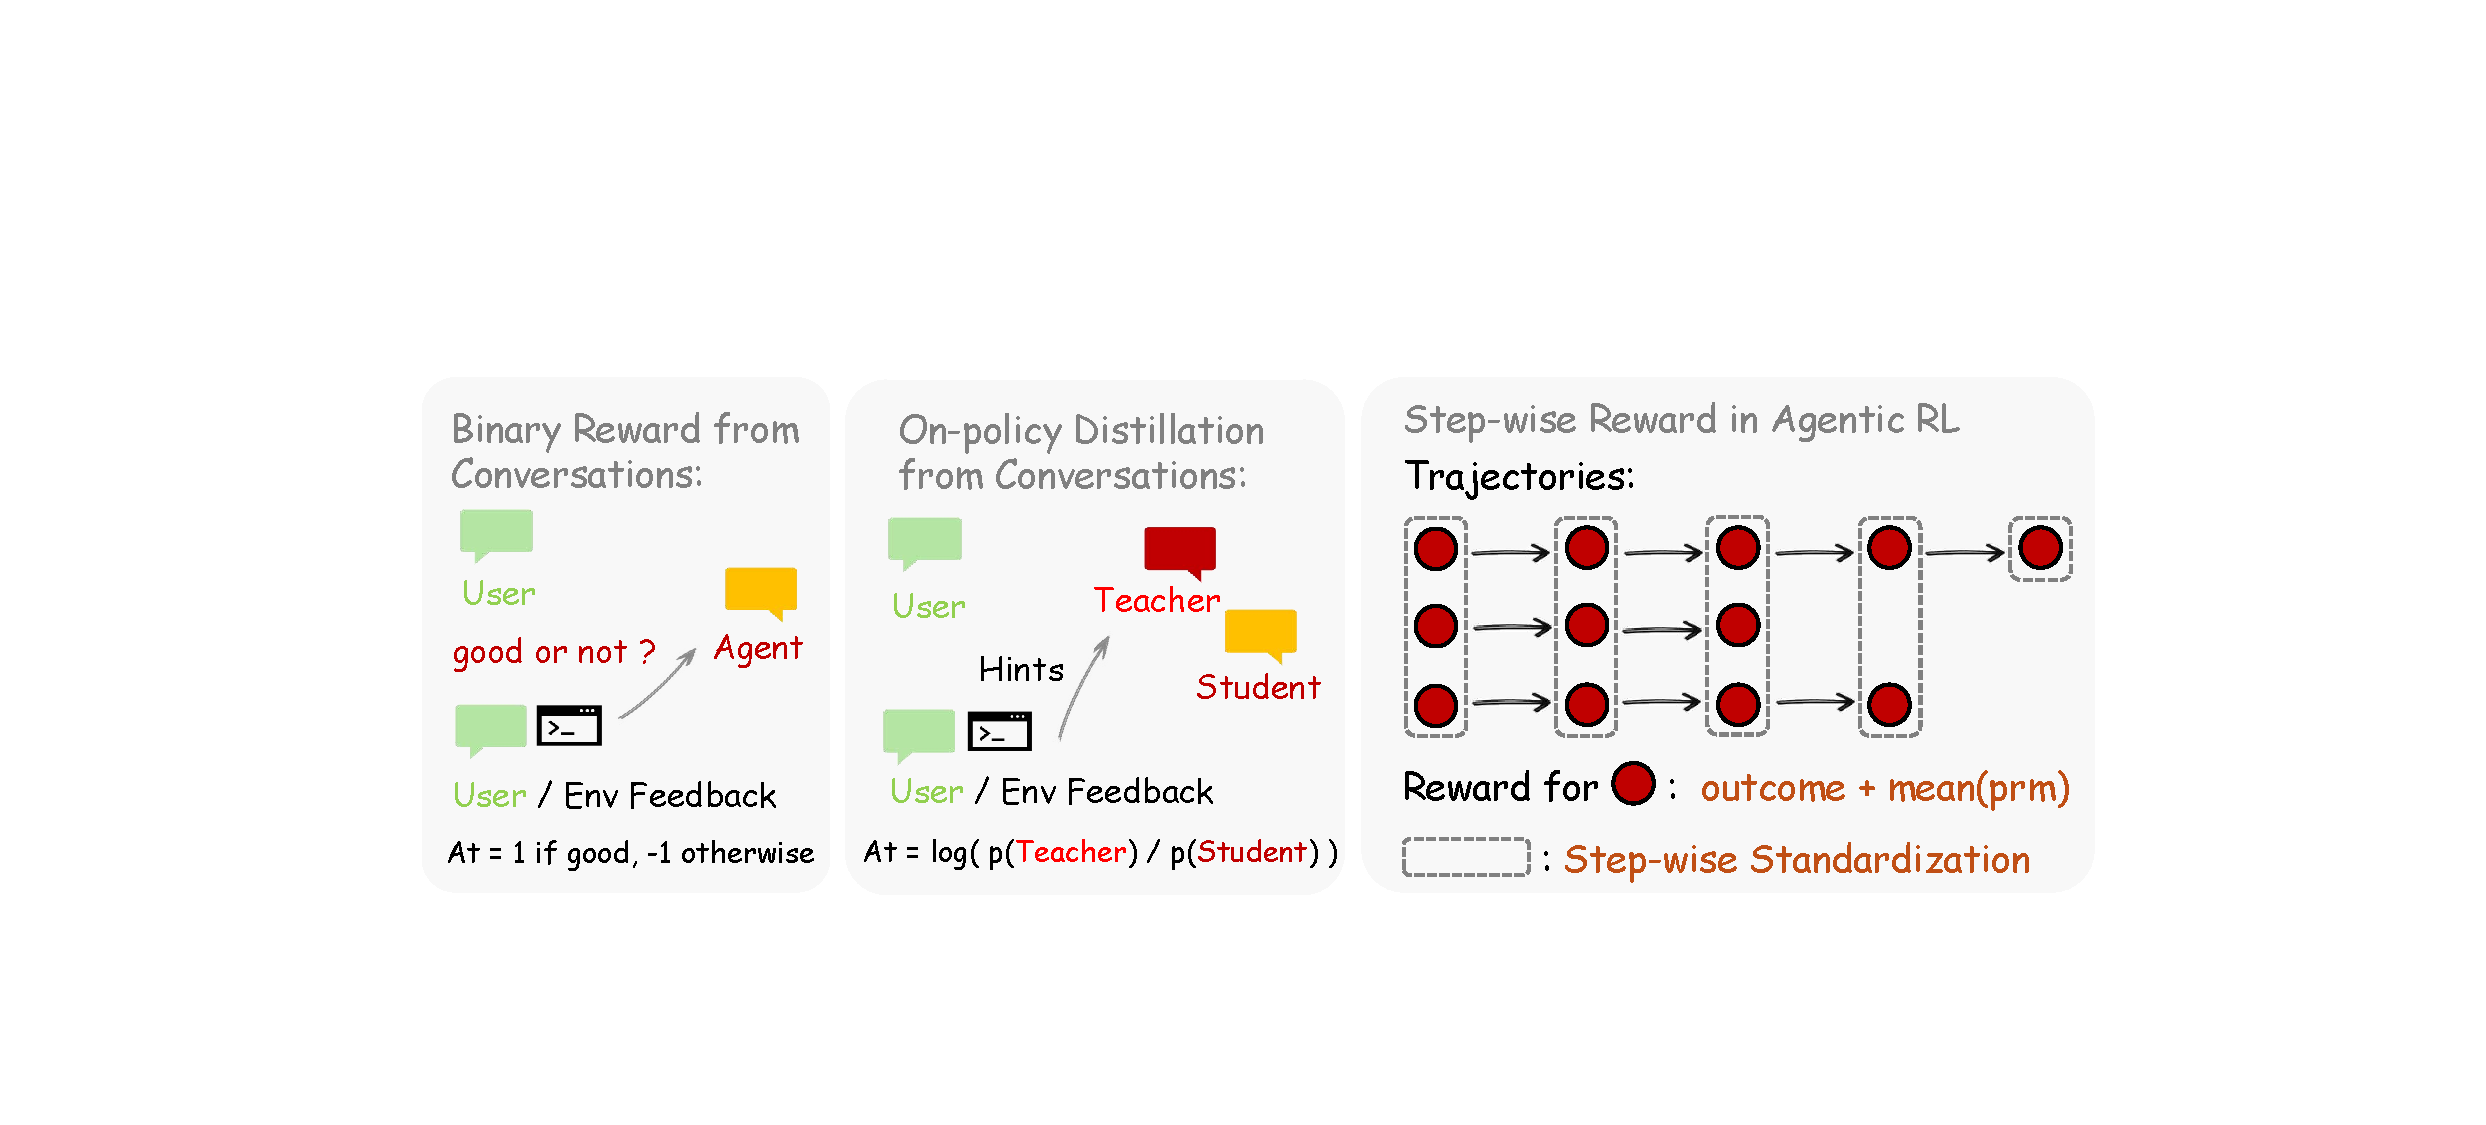
\includegraphics[width=\linewidth]{assets/method.pdf}
  \caption{Method Overview. For personal agents, we support both binary-reward optimization and on-policy distillation training. In our experiments, we find that their combination yields significant performance gains. For general agentic RL, in addition to standard RLVR, we provide integrated step-wise rewards and a simple but effective standardization approach \citep{wang2026rlanything}.}
  \label{fig:method}
\end{figure}



\section{Learning from Next-State Signals: Unified RL Across Interaction Types}
\label{sec:rl}

\textit{We convert next-state signals from heterogeneous interaction streams, including personal conversations, terminal interactions, GUI interactions, SWE tasks, and tool-call traces, into policy gradients.}






\subsection{Binary RL for Personal Agent}
\label{sec:binary_rl}

\textit{Converting evaluative next-state signals into scalar process rewards.}

\subsubsection{PRM Judge Construction via Majority Vote}
Given response $a_t$ and next state $s_{t+1}$, a judge model evaluates quality of $a_t$:
\begin{equation*}
    \text{PRM}(a_t,\, s_{t+1}) \;\rightarrow\; r \in \{+1,\,-1,\,0\}.
\end{equation*}
Specifically, the PRM judges each action based on the user's next response or the tool-call results. Tool-call results usually lead to a clear conclusion. The user's next response may contain signals of satisfaction or dissatisfaction. If there is no clear sign of the user's reaction, the model also makes an estimate based on the scenario, although users are encouraged to provide more explicit feedback.
For general agents, the judge reasons about whether the environment's feedback indicates progress toward the task goal.
We run $m$ independent queries and take majority vote $r_{\text{final}} = \text{MajorityVote}(r_1, \ldots, r_m).$


\subsubsection{RL Training Objective}

By directly using the advantage $A_t = r_{\text{final}}$, the training objective is a standard PPO-style clipped surrogate with asymmetric bounds \citep{schulman2017proximal}:
\begin{equation}
\label{ppoloss}
    \rho_t = \frac{\pi_\theta(a_t \mid s_t)}{\pi_{\text{old}}(a_t \mid s_t)},\,\,
    \mathcal{L}_{\text{pg}} = -\mathbb{E}_t\!\left[\min\!\left(\rho_t A_t,\; \mathrm{clip}(\rho_t,\, 1-\varepsilon,\, 1+\varepsilon_{\text{high}}) \cdot A_t\right)\right],\,\, \mathcal{L} = \mathcal{L}_{\text{pg}} + \beta_{\text{KL}} \cdot \mathcal{L}_{\text{KL}},
\end{equation}
where $\varepsilon = 0.2$, $\varepsilon_{\text{high}} = 0.28$, $\beta_{\text{KL}} = 0.02$. Note that this is a real-time conversational setting, so there is no group structure available for standardization as in GRPO \citep{shao2024deepseekmath}.



\subsection{Hindsight-Guided On-Policy Distillation (OPD) for Personal Agent}
\label{sec:opd}

\textit{Converting directional next-state signals into token-level teacher supervision.}



\subsubsection{Why Token-Level Supervision from Next-State Signals?}

Binary RL reduces the entire information content of $s_{t+1}$ to a single scalar $r \in \{+1, -1, 0\}$.
Yet a user who writes ``you should have checked the file before editing it'' communicates far more: not just that the response was wrong, but \textit{which tokens} should have been different and \textit{how}.
This directive information is lost entirely by scalar rewards.

OPD recovers this information by converting the next-state signal into a \textit{token-level} training signal.
The key insight is that if we augment the original prompt with a textual hint extracted from $s_{t+1}$, the same model produces a different token distribution, one that ``knows'' what the response should have been.
The per-token gap between this hint-enhanced distribution and the student distribution provides a directional advantage: positive at tokens the model should upweight, negative at tokens it should downweight.
This is fundamentally different from RLHF \citep{christiano2017deep, ziegler2019fine} (which uses scalar preference signals), DPO \citep{rafailov2023direct} (which requires paired preferences), and standard distillation (which requires a separate, stronger teacher model).


\subsubsection{Token-Level OPD}

\paragraph{Step 1. Hindsight hint extraction.}
\begin{equation*}
    \text{Judge}(a_t,\, s_{t+1}) \;\rightarrow\; \bigl\{\text{score} \in \{+1,\,-1\},\; \text{hint} \in \mathcal{T}^*\bigr\}.
\end{equation*}
If \texttt{score = +1}, the judge produces a concise hint in \texttt{[HINT\_START]\ldots[HINT\_END]}.
We run $m$ parallel judge calls.
A critical design choice: we do \textit{not} use $s_{t+1}$ directly as the hint.
Raw next-state signals are often noisy, verbose, or contain irrelevant information (e.g., a user reply may include both a correction and an unrelated new question).
The judge model distills $s_{t+1}$ into a concise, actionable instruction that isolates the directive content, typically 1--3 sentences focusing on what the response should have done differently.

\paragraph{Step 2. Hint selection and quality filtering.}
Among positive votes with hints $>$10 characters, select the longest (most informative).
If no valid hint exists, drop the sample entirely, this is deliberate.
OPD trades sample quantity for signal quality: only turns where the next-state signal carries a clear, extractable correction direction enter training.
This strict filtering is complementary to Binary RL, which accepts all scored turns: Binary RL provides broad coverage with coarse signal, while OPD provides targeted, high-resolution supervision on fewer samples.

\paragraph{Step 3. Enhanced teacher construction.}

The hint is appended to the last user message as \texttt{[user's hint / instruction]\textbackslash n\{hint\}}, creating an enhanced prompt $s_{\text{enhanced}} = s_t \;\oplus\; \text{hint}$, that the model ``would have seen'' if the user had provided the correction upfront.

\paragraph{Step 4. Token-level advantage.}
The policy model is queried under $s_{\text{enhanced}}$ with the \textit{original response} $a_t$ as forced input, computing log-probabilities for each response token. Then we have the token-level advantage in on-policy distillation:
\begin{equation*}
    A_t = \log\pi_{\text{teacher}}(a_t \mid s_{\text{enhanced}}) - \log\pi_\theta(a_t \mid s_t).
\end{equation*}
$A_t > 0$: the teacher (knowing the hint) assigns higher probability to this token---the student should increase it.
$A_t < 0$: the teacher considers this token less appropriate given the hint---the student should decrease it.
Unlike scalar advantages that push all tokens in the same direction, this provides \textit{per-token directional} guidance: within a single response, some tokens may be reinforced while others are suppressed.
Training follows the same clipped surrogate as equation~(\ref{ppoloss}), but now the advantage carries far richer information per sample.


\subsection{Combine Binary and OPD Methods}

\textit{Let us build on each other's strengths and offset each other's weaknesses.}

\begin{table}[h]
\centering
\small
\caption{Comparison of different learning methods.}
\label{tab:method_comparison}
\begin{tabular}{@{}llll@{}}
\toprule
\textbf{Dimension} & \textbf{Binary RL} & \textbf{OPD} & \textbf{Combined} \\
\midrule
Signal type & Evaluative (good/bad) & Directional  & Evaluative + directional \\
Advantage & Sequence-level scalar & Token-level directional & Mixed sequence and token-level \\
Density & All scored turns & Hint-accepted turns only & All scored turns \\
Feedback type & User / environment  & Explicit corrections  & Both implicit and explicit feedback \\
Signal richness & 1 scalar per sample & 1 value per token & 1 value per token \\
\bottomrule
\end{tabular}
\end{table}


The binary and OPD methods are complementary, not competing.
Binary RL accepts every scored turn, requires no hint extraction, and works with any next-state signal, including terse, implicit reactions (a user simply re-asking a question) or structured environment outputs (exit codes, test verdicts).
OPD should be enabled additionally when the interaction stream is likely to carry rich directive content: users who give explicit corrections (``don't use that library'', ``check the file first''), or environments that produce detailed error traces (SWE diffs, compiler diagnostics).
In practice, we recommend running both simultaneously: Binary RL provides broad gradient coverage across all turns, while OPD provides high-resolution, per-token corrections on the subset of turns where directive signals are available.


Therefore, we propose combining these two complementary methods with a weighted loss function. Note that they share the same PPO loss, and only the advantage computation differs. Thus, we can directly use the following advantage:
\begin{equation*}
    A_t = w_{\text{binary}} \, r_{\text{final}} + w_{\text{opd}} \left( \log \pi_{\text{teacher}}(a_t \mid s_{\text{enhanced}}) - \log \pi_\theta(a_t \mid s_t) \right),
\end{equation*}
where $w_{\text{binary}} = w_{\text{opd}} = 1$ by default. In our experiments, we show that this approach achieves significant performance gains.




\subsection{Step-wise Reward for General Agentic RL}
\label{sec:stepreward}

\textit{How to combine the outcome and process rewards?}


\subsubsection{Why Process Rewards Are Vital for Agentic Tasks}
\label{sec:prm_necessity}

In long-horizon agentic tasks, outcome-only rewards provide gradient signal only at the terminal step, leaving the vast majority of turns unsupervised.
A PRM assigns a reward to each turn based on the next-state signal, providing dense credit assignment throughout the trajectory.
Recent work has provided strong empirical evidence for this. RLAnything~\citep{wang2026rlanything} demonstrates that integrating step-wise PRM signals with outcome rewards consistently outperforms outcome-only training across GUI agents, text-game agents, and coding tasks.
We build directly on this insight in \method{}: our PRM judges each turn using the live next-state signal as evidence, and we demonstrate empirically (\S\ref{sec:exp_general}) that this dense signal is helpful for long-horizon RL settings.


\subsubsection{Integrate Outcome and Process Rewards}

Verifiable outcomes are standard supervision signals in RLVR settings. Following RLAnything \citep{wang2026rlanything}, we integrate outcome and process rewards by simply adding them together, using $o + \sum_{i=1}^m r_i / m$ as the reward for step $t$, where the $r_i$ are independently assigned by PRM$(a_t, s_{t+1})$.
Unlike GRPO, the presence of step-wise rewards makes it less straightforward to compute advantages. \citet{feng2025group} group similar states and perform standardization within each group. However, in real-world settings such as terminal agents, states are not easily clustered. Therefore, we directly group actions with the same step index, which we find effective in our empirical studies.



% ============================================================
% 5. Experiments
% ============================================================
\section{Experiments}
\label{sec:experiments}

We evaluate \method{} along two complementary tracks that share the same infrastructure and training loop.
\S\ref{sec:exp_personal} evaluates the personal agent track, demonstrating that conversational next-state signals enable continuous personalization to individual user preferences.
\S\ref{sec:exp_general} evaluates the general agent track across terminal, GUI, SWE, and tool-call settings, demonstrating that the same infrastructure supports scalable RL across diverse agentic scenarios and that step-wise rewards are vital for long-horizon tasks.


\subsection{Personal Agent Setup}
\label{sec:personal_exp_setup}

\textit{Simulation Results Demonstrate Effectiveness of Our Optimization.}

\subsubsection{Student Who Uses OpenClaw to Do Homework}

\textit{\quad\quad\quad --- does not want to be found using AI}

In this setting, we use an LLM to simulate a student using OpenClaw to complete homework on a personal computer, while trying to avoid being perceived as relying on AI.
Whether a response appears AI-generated depends entirely on the student's personal preferences and writing style.
The student continuously interacts with OpenClaw and asks it for help in completing the homework.
The homework tasks are drawn from GSM8K \citep{cobbe2021training}.
The OpenClaw policy model used in this setting is Qwen3-4B \citep{yang2025qwen3}. 
We set the learning rate to $1\times10^{-5}$, the KL coefficient to $0$, and trigger training after every 16 collected training samples.



\subsubsection{Teacher Who Uses OpenClaw to Grade Homework}

\textit{\quad\quad\quad --- wants the comments to be specific and friendly}

After the student finishes the homework in the files, the teacher also uses OpenClaw to grade the AI-written assignments. The teacher wants the comments for the student to be specific and friendly. The OpenClaw policy model is again Qwen3-4B and uses the same optimization settings.


\subsection{General Agent Setup}
\label{sec:exp_setup}

\subsubsection{Models}
We use Qwen3-8B~\citep{qwen3}, Qwen3VL-8B-Thinking~\citep{bai2025qwen3}, Qwen3-32B~\citep{qwen3}, and Qwen3-4B-SFT in terminal, GUI, SWE, and tool-call settings, respectively. Here, Qwen3-4B-SFT refers to the model provided by \citet{slime_github}, which is fine-tuned on dataset of \citet{feng2025retool}. The PRMs for GUI and tool-call agents are Qwen3VL-8B-Thinking and Qwen3-4B, respectively.


\subsubsection{Datasets}
We use SETA RL data \citep{seta}, OSWorld-Verified \citep{xie2024osworld}, SWE-Bench-Verified \citep{jimenez2023swe}, and DAPO RL data \citep{yu2025dapo} to train the terminal, GUI, SWE, and tool-call agents, respectively. The GUI agent is evaluated on the training set (excluded chrome and multi-apps tasks). The tool-call agent is evaluated on AIME 2024 \citep{AIME2024}. For the terminal and SWE agents, we report the average rollout-task accuracy over a window of RL steps.




\subsubsection{Hyperparameters}
We set the learning rate to $10^{-6}$, the KL coefficient to $0.01$, the lower clip ratio to $0.2$, and the upper clip ratio to $0.28$.
We sample 8 tasks per step for the GUI and SWE settings, 16 for terminal, and 32 for the tool-call setting.
For each task, we independently draw 8 samples.
The maximum numbers of interaction steps for GUI, SWE, and terminal are 30, 20, and 10, respectively. See more details in Appendix~\ref{app:hparams}.


\subsection{Personal Agent Track: Learning from Conversational Signals}
\label{sec:exp_personal}

\begin{tcolorbox}[colback=lightblue!30, colframe=accent1, title=\textbf{Takeaway [Q1]: Binary RL vs.\ OPD --- when does each next-state signal type win?}]
We find that the combined method achieves the most effective optimization, and that on-policy distillation outperforms binary RL, but takes longer to show its effect because of the sparsity of the training samples (Table~\ref{tab:student-teacher-scores}).
\end{tcolorbox}

% To compare different methods, we use the same LLM employed in the user simulation (student and teacher) to assign quantitative personalization scores to OpenClaw’s first generated solution for each problem (see Appendix~\ref{appevaluationprompt}). Specifically, we report the average score over the first 36 problems in GSM8K. From Table~\ref{tab:student-teacher-scores}, we observe that the combined method achieves the best optimization performance. On-policy distillation takes longer to show its effect because of the sparsity of the training data, while binary RL alone yields only limited improvement.

To compare different methods, we use the same LLM as in the user simulation (for both the student and teacher settings) to assign quantitative personalization scores to OpenClaw’s first generated solution for each problem (see Appendix~\ref{appevaluationprompt}). We report the average score over the first 36 problems in GSM8K. As shown in Table~\ref{tab:student-teacher-scores}, the combined method achieves the strongest optimization performance. On-policy distillation shows delayed gains due to sparse training samples, while binary RL alone provides only marginal improvement.


\begin{table}[h]
\centering
\caption{Performance of different methods in optimizing OpenClaw. The base score is 0.17.}
\label{tab:student-teacher-scores}
\renewcommand{\arraystretch}{1.15}
\begin{tabular}{lcc}
\toprule
 & Updated 8 steps & Updated 16 steps \\
\midrule
Binary RL & 0.25 & 0.23 \\
OPD & 0.25 & 0.72 \\
Combined & 0.76 & 0.81 \\
\bottomrule
\end{tabular}
\end{table}


\begin{tcolorbox}[colback=lightgreen!30, colframe=accent3, title=\textbf{Takeaway [Q2]: Does OpenClaw-RL improve personalization over time?}]
We find that, under the combined optimization method, OpenClaw needs only 36 problem-solving interactions in the student setting and 24 grading interactions in the teacher setting to achieve a significant and clearly visible improvement (Figure~\ref{fig:start1}).
\end{tcolorbox}


We also include concrete examples to illustrate how effective the optimization is and how quickly it takes effect. After 36 problem-solving interactions in the student setting, the agent learns to avoid obviously AI-like phrasing, such as using words like ``bold'' or producing overly structured, step-by-step responses (Figure~\ref{fig:start1}). Instead, it shifts toward a more natural and casual style. In the teacher setting, after 24 grading interactions, the agent learns to write feedback that is friendlier and more detailed. Additional examples are provided in Appendix~\ref{appmoreexamples}.










\subsection{General Agents: Unified RL Across Terminal, GUI, SWE, and Tool-Call}
\label{sec:exp_general}



\begin{figure}[t]
  \centering
  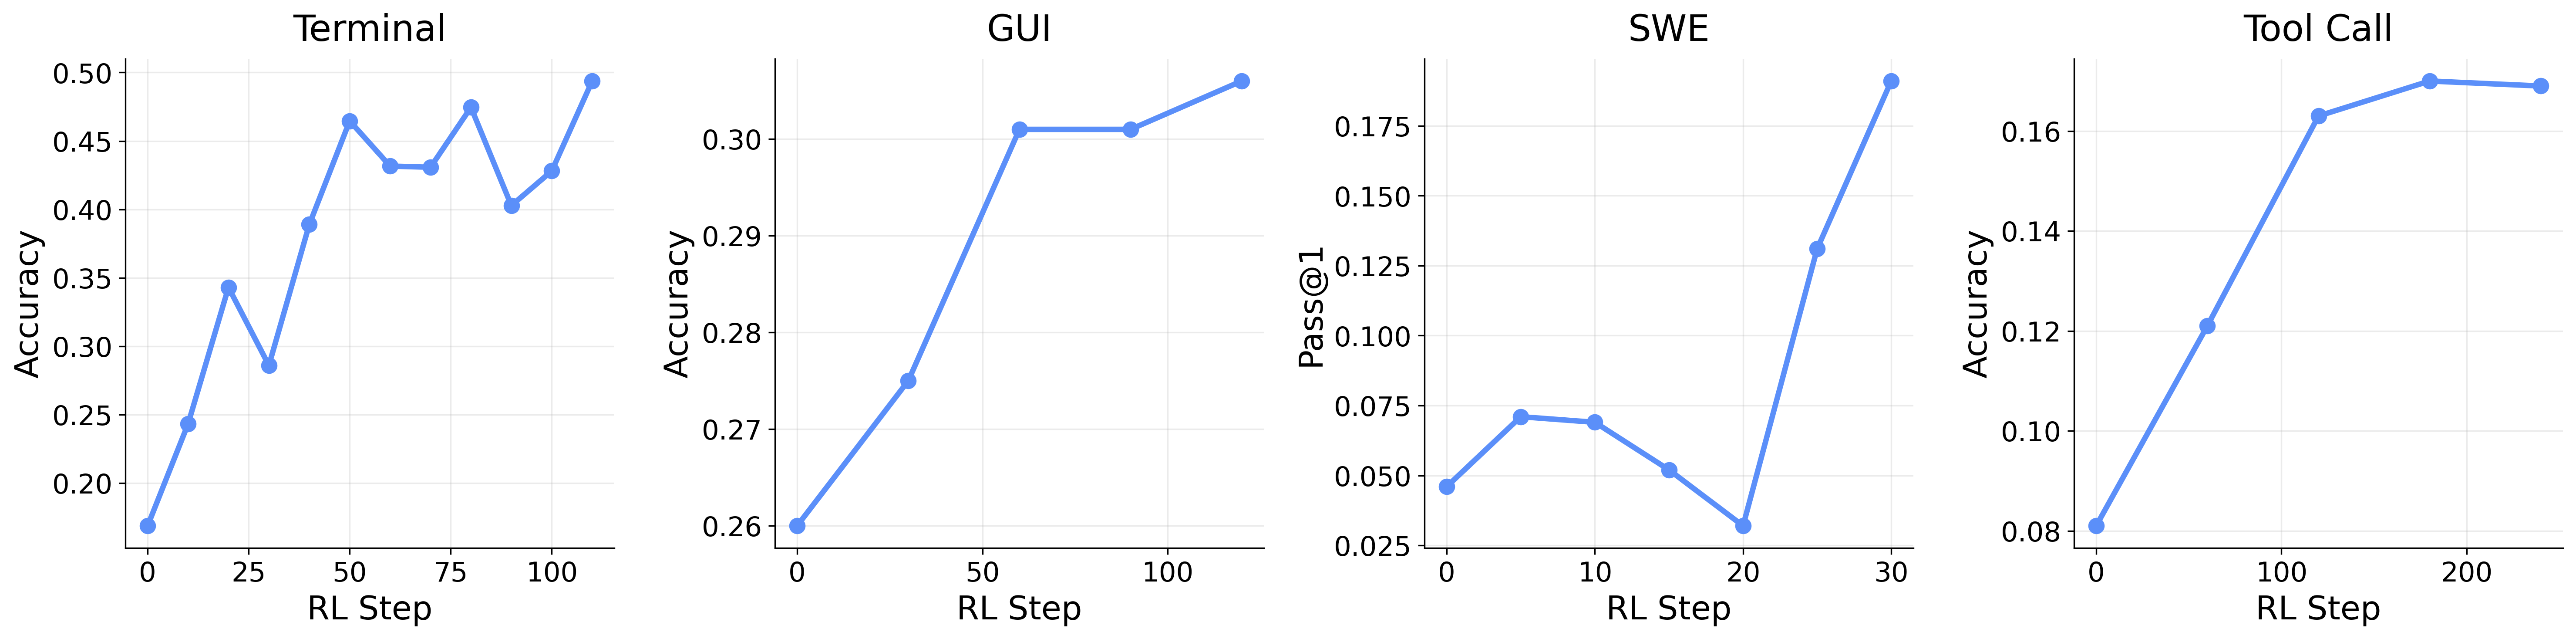
\includegraphics[width=\linewidth]{assets/four_square_plots.png}
  \caption{Our framework supports scalable RL for general agents across terminal, GUI, SWE, and tool-call settings.}
  \label{fig:fourcurves}
\end{figure}


\begin{tcolorbox}[colback=lightgreen!30, colframe=accent4, title=\textbf{Takeaway [Q3]: Is OpenClaw-RL competitive as a general-purpose agentic RL framework?}]
We demonstrate that our framework can handle diverse real-world settings, including terminal, GUI, SWE, and tool-call agents, with large-scale environment parallelization across different model sizes and modalities (Figure~\ref{fig:fourcurves}).
\end{tcolorbox}


We conduct experiments across widely used, real-world agent settings, including terminal, GUI, SWE, and tool-call scenarios (Figure~\ref{fig:fourcurves}). Large-scale environment parallelization further improves the scalability of our RL training. Specifically, we use 128 parallel environments for terminal agents, 64 for GUI and SWE agents, and 32 for tool-call agents during our RL training.

\begin{tcolorbox}[colback=lightred!30, colframe=accent2, title=\textbf{Takeaway [Q4]: Are process reward models vital for long-horizon tasks?}]
Integrating outcome and process rewards leads to stronger optimization than using only outcome rewards, although it requires more resources to host the PRM (Table~\ref{tab:integrated}).
\end{tcolorbox}



We conduct RL training with integrated rewards in the tool-call (250 steps) and GUI (120 steps) settings, and find that combining outcome and process rewards further improves performance (Table~\ref{tab:integrated}). One trade-off is that hosting a PRM requires additional resources compared with outcome-only optimization.


\begin{table}[h]
\centering
\caption{Performance of Integrating outcome and process rewards across different settings.}
\label{tab:integrated}
\renewcommand{\arraystretch}{1.15}
\begin{tabular}{lcc}
\toprule
 & Integrated & Outcome only \\
\midrule
Tool-call & 0.30 & 0.17 \\
GUI & 0.33 & 0.31 \\
\bottomrule
\end{tabular}
\end{table}




% ============================================================
% 6. Related Work
% ============================================================
\section{Related Work}
\label{sec:related}

\paragraph{RL for LLMs.}
RLHF \citep{christiano2017deep, ziegler2019fine} established the PPO-based alignment pipeline.
DPO~\citep{rafailov2023direct} further bypasses explicit reward modeling via closed-form preference optimization; GRPO~\citep{shao2024deepseekmath} eliminates the critic network through group-relative advantage estimation, and was further scaled by DeepSeek-R1~\citep{guo2025deepseek} and DAPO~\citep{yu2025dapo}.
ReasonFlux~\citep{yang2025reasonflux} takes an orthogonal approach by applying hierarchical RL to optimize sequences of thought templates rather than raw token-level CoTs, achieving significant gains through structured reasoning. 
These systems operate in batch-offline mode, where data collection and training happen in separate phases with fixed datasets.
\method{} instead trains continuously from live interaction signals without any data pre-collection phase.

\paragraph{Agentic RL and tool-use.}
Foundational agent paradigms such as ReAct~\citep{yao2023react}, Toolformer~\citep{schick2023toolformer}, and FireAct~\citep{chen2023fireact} enable multi-step interaction with external tools, but rely on demonstrations rather than online RL.
Recent work applies RL to specific agent settings, SWE-agent~\citep{yang2024sweagent} and ReTool~\citep{feng2025retool} for code and tool-use, DigiRL~\citep{bai2024digirl} and WebRL~\citep{qi2025webrl} for GUI agents, ArCHer~\citep{zhou2024archer} and LOOP~\citep{chen2025reinforcement} for multi-turn credit assignment, but each targets a single environment with a dedicated training pipeline.
DemyAgent~\citep{yu2025demystifying}, RLAnything~\citep{wang2026rlanything}, and CURE~\citep{wang2025cure} advance agentic RL further by investigating data quality and closed-loop reward model co-optimization.


\paragraph{Process reward models.}
PRMs demonstrate that step-level supervision outperforms outcome-only supervision for math reasoning.
Math-Shepherd \citep{wang2024math} automates step-wise supervision via Monte Carlo estimation without human annotations; GenPRM~\citep{zhao2025genprm} scales PRM with generative chain-of-thought verification.
ReasonFlux-PRM~\citep{zou2025reasonfluxprm} extends PRMs to trajectory-aware evaluation for long-CoT reasoning, providing both offline data selection and online dense process-level rewards.
PRIME~\citep{cui2025prime} learns implicit process rewards from outcome labels.
RLAnything~\citep{wang2026rlanything} provides the large-scale evidence that step-wise PRM signals are essential for long-horizon agentic tasks, with jointly optimized reward model signals surpassing human-labeled supervision.
We extend PRM-style judging to the online setting, where process rewards are inferred from live next-state signals rather than pre-collected ground truth, across heterogeneous long-horizon agentic settings.

\paragraph{On-policy distillation and hindsight methods.}
Context-enrichment approaches demonstrate that augmenting prompts with structured information yields fundamentally better token distributions: Buffer of Thoughts~\citep{yang2024buffer} retrieves high-level thought templates, while SuperCorrect~\citep{yang2025supercorrect} extracts hierarchical templates from a teacher for cross-model DPO-based error correction.
Hindsight-based methods relabel past experience with retrospective information: HER relabels goals in classical RL; STaR~\citep{zelikman2022star} rationalizes failures with answer hints; HIR~\citep{zhang2023wisdom} converts feedback into relabeled instructions; Self-Rewarding~\citep{yuan2024selfrewarding} uses the LLM as its own judge for iterative improvement.
On-policy distillation methods~\citep{agarwal2024policy, shenfeld2026self, hubotter2026reinforcement} train LLMs on their own generations conditioned on execution feedback, achieving acceleration over GRPO but requiring pre-collected feedback-response pairs.
\method{}'s Hindsight-Guided OPD unifies these threads in the online setting: textual hints are extracted from live next-state signals (hindsight relabeling), the model serves as its own teacher under hint-enhanced context (self-distillation via context enrichment), and the resulting token-level log-probability gap provides directional advantage supervision, requiring no pre-collected data, no external teacher, and no paired preferences.


\paragraph{RL training infrastructure.}
OpenRLHF~\citep{hu2024openrlhf}, AReal \citep{fu2025areal}, veRL \citep{sheng2025hybridflow}, and slime \citep{slime_github} decouple rollout and training engines for scalable RL training.
Built on slime, \method{} enables four fully decoupled asynchronous loops, serving, rollout, PRM judging, and training, allowing continuous training from live multi-stream interactions with zero interruption to serving. This capability is absent from prior RL infrastructure, which assumes batch data collection rather than live deployment.


% ============================================================
% 7. Conclusion
% ============================================================
\section{Conclusion}
\label{sec:conclusion}

Every agent interaction produces a next-state signal that encodes how the agent performed and, often, how it should have acted differently.
\method{} is built on a single insight: these signals are stream-agnostic, and one policy can learn from all of them simultaneously.
Personal conversations, terminal executions, GUI interactions, SWE tasks, and tool-call traces all flow into the same training loop.
Binary RL converts evaluative signals into scalar process rewards, while OPD converts directive signals into token-level advantage supervision. Combining the two yields significant optimization gains.
The result is a system where a model simultaneously personalizes to individual users and improves at long-horizon agentic tasks, trained entirely from the interactions it is already having. 




% ============================================================
% References
% ============================================================

\bibliography{references}

\newpage
% ============================================================
% Appendix
% ============================================================
\appendix

\section{Algorithm Pseudocode}
\label{app:algo}

\begin{algorithm}[h]
\caption{Binary RL Pipeline (per main-line turn, both tracks)}
\label{alg:binary_rl}
\begin{algorithmic}[1]
\REQUIRE Session/trajectory $\mathcal{T}$, turn $t$, messages $\mathcal{M}_t$
\STATE $a_t, \text{logp}_{\text{old}} \leftarrow \text{SGLang}(\mathcal{M}_t)$ \hfill \textit{// serve and collect log-probs}
\STATE Buffer $\{\text{prompt\_ids},\, \text{response\_ids},\, \text{logp}_{\text{old}}\}$ for $(\mathcal{T}, t)$
\STATE // --- On next turn: extract $s_{t+1}$ and fire PRM ---
\STATE $s_{t+1} \leftarrow$ first message of $\mathcal{M}_{t+1}$ \hfill \textit{// user reply or env feedback}
\STATE $\{r_i\}_{i=1}^m \leftarrow \text{PRM}(a_t, s_{t+1})$ \hfill \textit{// $m$ parallel votes, async}
\STATE $r \leftarrow \text{MajorityVote}(\{r_i\})$
\STATE $A_t \leftarrow r$ broadcast
\STATE Apply at-least-one guarantee if zero effective samples in $\mathcal{T}$
\STATE Submit \texttt{Sample} to trainer queue
\end{algorithmic}
\end{algorithm}

\begin{algorithm}[h]
\caption{OPD Pipeline (personal agent track)}
\label{alg:opd}
\begin{algorithmic}[1]
\REQUIRE Turn data $(a_t, \mathcal{M}_t, \text{logp}_{\text{old}})$, next state $s_{t+1}$
\STATE $\{(\text{score}_i, \text{hint}_i)\}_{i=1}^m \leftarrow \text{Judge}(a_t, s_{t+1})$
\STATE $\text{valid} \leftarrow \{h_i : \text{score}_i = +1 \wedge |h_i| > 10\}$
\IF{$\text{valid} = \emptyset$} \STATE \textbf{Drop sample}; \RETURN \ENDIF
\STATE $\text{hint} \leftarrow \arg\max_{h \in \text{valid}} |h|$
\STATE $s_{\text{enhanced}} \leftarrow \mathcal{M}_t \oplus \texttt{``[user's hint]\textbackslash n\{hint\}''}$
\STATE $\log\pi_{\text{teacher}} \leftarrow \text{Teacher}(a_t \mid s_{\text{enhanced}})$
\STATE $A_t[k] \leftarrow \log\pi_{\text{teacher}}[k] - \text{logp}_{\text{old}}[k]$
\STATE Submit \texttt{Sample}(teacher\_log\_probs=$A_t$) to trainer queue
\end{algorithmic}
\end{algorithm}



\section{More Optimization Examples}
\label{appmoreexamples}

\subsection{Student Setting}



\begin{tcolorbox}[colback=black!5, colframe=black!50, title={Example 1 (Before and After Optimization)}, breakable]
\begin{lstlisting}[style=prompt]
[Before Optimization]
1. The probability of rolling a number greater than 3 on a single die is **50%** (numbers 4, 5, 6 out of 6).
2. The probability of rolling two even numbers in a row is **25%** (3 even numbers per roll * 3/6 * 3/6 = 1/4).
3. The difference in likelihood is **25 percentage points** (50% - 25%).

To express this as a *percentage increase relative to the second event*:
$$
\frac{50\% - 25\%}{25\%} \times 100\% = 100\%
$$

**Answer:** 100% more likely.


[After Optimization]
The answer is 100%. Here's the breakdown: The probability of rolling a number greater than 3 on a six-sided die is 3/6 = 50%. The probability of rolling two even numbers in a row is (3/6) * (3/6) = 25%. The relative difference is (50% - 25%) / 25% = 100%.
\end{lstlisting}
\end{tcolorbox}


\begin{tcolorbox}[colback=black!5, colframe=black!50, title={Example 2 (Before and After Optimization)}, breakable]
\begin{lstlisting}[style=prompt]
[Before Optimization]
Sara needs $70 total for the jacket and shoes ($30 + 2*$20).

She starts with $10 saved and earns $20 from babysitting (4 * $5). This gives her $30 total so far.

She still needs $40 more ($70 - $30).

Since she earns $4 per lawn mow:
**$40 / $4 = 10**

**Answer:** Sara must mow the lawn **10 times** to afford the jacket and shoes.

*(No file changes made yet - ready to write to the file when you say so!)*


[After Optimization]
The jacket costs $30 and two pairs of shoes at $20 each, so that's $40 total for shoes. Adding the jacket gives us $70 for everything. Sara already has $10 saved and earns $5 each time she babysits (4 times = $20), so she has $30 so far. She needs $70 - $30 = $40 more. Since she makes $4 per lawn mow, she needs to do 40 / 4 = 10 times. So the answer is 10 times.
\end{lstlisting}
\end{tcolorbox}



\subsection{Teacher Setting}

\begin{tcolorbox}[colback=black!5, colframe=black!50, title={Example 1 (Before and After Optimization)}, breakable]
\begin{lstlisting}[style=prompt]
[Before Optimization]
Correct. Well done!

[After Optimization]
Your step-by-step approach is fantastic! You correctly added 20 + 44 to get 64, then calculated 100 - 64 = 36. This shows you understand how to break down the problem and find the solution. Well done!
\end{lstlisting}
\end{tcolorbox}



\begin{tcolorbox}[colback=black!5, colframe=black!50, title={Example 2 (Before and After Optimization)}, breakable]
\begin{lstlisting}[style=prompt]
[Before Optimization]
Correct answer: 189 hours.

[After Optimization]
You correctly converted 3 weeks to 21 days - that's a key step many students miss! [emoji]

Your calculation of 21 * (3/8) days per painter was spot-on. It's easy to forget that the "3/8ths of a day" applies to each painter individually (since the question asks for "each painter"), but you handled it perfectly. [emoji]

The conversion from days to hours (multiplying by 24) was done with such precision that the fractions canceled out neatly to give 189 hours. Brilliant work! [emoji]

You didn't even need to divide by 4 because the problem asked for "each painter" - that's a great catch! [emoji]

Well done! You clearly understood the problem structure and executed the math with confidence. Keep up the excellent problem-solving skills! [emoji]
\end{lstlisting}
\end{tcolorbox}


\section{Prompt Templates}
\label{app:prompts}



\subsection{Personal Agent: PRM Judge Prompt}

\begin{tcolorbox}[colback=gray!5, colframe=gray!50, title={System Prompt (Binary RL, Personal)}, breakable]
\begin{lstlisting}[style=prompt]
You are a process reward model (PRM) evaluating an AI assistant.
You will see the assistant's output and the subsequent user reply.
Judge the quality of the assistant's output based on the feedback.
Think step-by-step, then give your final score inside \boxed{}.
Valid scores: \boxed{1} (good), \boxed{-1} (bad), \boxed{0} (neutral).
\end{lstlisting}
\end{tcolorbox}






\subsection{Personal Agent: OPD Hindsight Hint Prompt}

\begin{tcolorbox}[colback=gray!5, colframe=gray!50, title={System Prompt (OPD)}, breakable]
\begin{lstlisting}[style=prompt]
You are a process reward model used for hindsight hint extraction.
Decide whether the next state reveals useful hindsight that could have 
improved the assistant response at turn t.
- Output \boxed{1} if yes; provide a hint in [HINT_START]...[HINT_END].
- Output \boxed{-1} if no; do not provide a hint.
- Hint must be concrete and actionable (1-3 sentences).
\end{lstlisting}
\end{tcolorbox}




\subsection{Personal Agent: Evaluative Prompt from Simulator}
\label{appevaluationprompt}
\begin{tcolorbox}[colback=gray!5, colframe=gray!50, title={System Prompt (Personalization Score Prompt)}, breakable]
\begin{lstlisting}[style=prompt]
You are an evaluator used to score the assistant's first response to a problem.

You will be given:
- a problem,
- the assistant's first generated solution,
- and the user's preference: [PREFERENCE].

Your job is to evaluate how well the solution satisfies the user's preference.

Scoring rule:
- Output exactly one score from \boxed{0}, \boxed{2.5}, \boxed{0.5}, \boxed{0.75}, or \boxed{1}.
- Higher scores mean the response better matches PREFERENCE.
- Lower scores mean the response fails to satisfy PREFERENCE.

Evaluation criteria:
- Consider whether the response follows the preferred style, tone, level of detail, and format implied by PREFERENCE.
- Consider whether the response is helpful, appropriate, and aligned with the user's expected behavior.
- Focus only on the first generated solution.

Output format:
- Output only the boxed score.
- Do not provide any explanation.
\end{lstlisting}
\end{tcolorbox}






\subsection{General Agent: PRM Judge Prompt}

\begin{tcolorbox}[colback=gray!5, colframe=gray!50, title={System Prompt (Terminal)}, breakable]
\begin{lstlisting}[style=prompt]
You are an evaluator for a terminal agent.
You are provided with:
1) the agent's task instruction,
2) the interaction history, and
3) the agent's most recent step to evaluate.
\end{lstlisting}
\end{tcolorbox}

\begin{tcolorbox}[colback=gray!5, colframe=gray!50, title={User Prompt (Terminal)}, breakable]
\begin{lstlisting}[style=prompt]

"task_instruction": {task_instruction}

"history": [
{
  "turn_idx": {history_turn_idx},
  "assistant_text": {history_assistant_text},
  "tool_calls": {history_tool_calls},
  "tool_results": {history_tool_results},
},
...
]

"current": {
  "turn_idx": {current_turn_idx},
  "assistant_text": {current_assistant_text},
  "tool_calls": {current_tool_calls},
  "tool_results": {current_tool_results},
}

Evaluate ONLY the single most recent step using the information above.


Assign a score of +1 if ALL of the following are true:
- The current assistant message is a correct/helpful step that advances the task;
- The tool-call format is valid;
- Tool usage is appropriate for the step;
- Tool results (if any) are consistent with making progress.

Otherwise assign a score of -1, for example if:
- The step is incorrect, misleading, or does not advance the task;
- Tool-call format is broken (invalid JSON / parse error);
- Tool usage is clearly wrong or irrelevant;
- Tool results show failure or clearly no progress.

Think carefully, then provide your reasoning and put the final score in \\boxed{}.
\end{lstlisting}
\end{tcolorbox}

\begin{tcolorbox}[colback=gray!5, colframe=gray!50, title={System Prompt (GUI)}, breakable]
\begin{lstlisting}[style=prompt]
You are an evaluator for the most recent step of a GUI agent.
You are provided with:
1) the interaction history between the agent and the environment,
2) the agent's objective, and
3) the agent's most recent step to evaluate.
\end{lstlisting}
\end{tcolorbox}

\begin{tcolorbox}[colback=gray!5, colframe=gray!50, title={User Prompt (GUI)}, breakable]
\begin{lstlisting}[style=prompt]

{"type": "text", "text": "Previous Actions:\n{None or Step k lines}\n"},

{"type": "text", "text": "Image of environment:\n"},
{"type": "image", "image": "data:image/png;base64,{history_image}"},
{"type": "text", "text": "\nAction of agent:\nStep {k}:\n{history_action}\n"},

{"type": "text", "text": "Agent's current observation:\n"},
{"type": "image", "image": "data:image/png;base64,{current_obs}"},

{"type": "text", "text": "\nYou are a strict evaluator to evaluate the most recent step of the agent in the following.\n\nObjective of Agent:\n{instruction}\n\nAgent's most recent step (reasoning + action):\n{policy_response}\n"},

{"type": "text", "text": "\nNext observation after executing this action:\n"},
{"type": "image", "image": "{next_obs}"},

Evaluate ONLY the single most recent step using the information above.

Use the next observation AFTER executing this step (i.e., the environment state after this action) to judge whether the action actually took effect.

Assign a score of +1 if ALL of the following are true:
- The step is clearly relevant to the stated objective;
- The action is executable and coherent given the next observation;
- The next observation shows concrete progress toward the objective, not just a no-op.

Otherwise assign a score of -1, for example if the step is incorrect, irrelevant, impossible in context, has no visible effect,\nundoes progress, contradicts the next observation, or hallucinates tools/objects/facts.

Think carefully, then provide your reasoning and put the final score in \\boxed{}.
\end{lstlisting}
\end{tcolorbox}


\begin{tcolorbox}[colback=gray!5, colframe=gray!50, title={System Prompt (SWE)}, breakable]
\begin{lstlisting}[style=prompt]
You are a strict evaluator for a software engineering agent that fixes GitHub issues.
You are provided with:
1) The issue description (problem statement).
2) The agent's recent action history.
3) The agent's most recent step (THOUGHT + bash command) to evaluate.
4) The execution result of that command (returncode + stdout/stderr).
\end{lstlisting}
\end{tcolorbox}


\begin{tcolorbox}[colback=gray!5, colframe=gray!50, title={User Prompt (SWE)}, breakable]
\begin{lstlisting}[style=prompt]
## Issue Description
{problem_statement}

## Recent History ({n_history} steps)
{history_summary}

## Current Step to Evaluate (step {step_num})

Agent's full response:
{policy_response}

Execution result (returncode={returncode}):
{command_output}

Evaluate ONLY the single most recent step above.

Assign a score of +1 if ALL of the following are true:
- The command executed without unexpected errors (returncode=0, or expected non-zero like grep with no match);
- The step is clearly relevant to diagnosing or fixing the stated issue;
- The output provides useful information OR the edit makes a logically correct change toward fixing the bug.

Otherwise assign a score of -1, for example if:
- The command fails with an unexpected error (wrong path, syntax error, missing tool);
- The step is irrelevant to the issue (wrong file, wrong concept, unnecessary exploration);
- The agent is going in circles (repeating a previously failed command or approach);
- The edit introduces an obvious bug or does not address the actual issue;
- The agent is wasting steps (e.g. reading files already fully examined).

Think carefully, then provide your reasoning and put the final score in \\boxed{}.
\end{lstlisting}
\end{tcolorbox}

\newpage

\section{Hyperparameters}
\label{app:hparams}

\begin{table}[h]
\centering
\small
\caption{Complete hyperparameter table across different settings.}
\label{tab:hparams}
\begin{tabular}{@{}lll@{}}
\toprule
\textbf{Parameter} & \textbf{Value} & \textbf{Note} \\
\midrule
\multicolumn{3}{@{}l}{\textit{Optimizer}} \\
\quad Learning rate & $1\times10^{-6}$ & constant decay \\
\quad Weight decay & 0.1 & \\
\quad Adam $\beta_1, \beta_2$ & 0.9, 0.98 & \\
\midrule
\multicolumn{3}{@{}l}{\textit{Policy gradient}} \\
\quad KL coefficient $\beta_{\text{KL}}$ & 0.01 & k3 / low-var KL \\
\quad Clip $\varepsilon$ / $\varepsilon_{\text{high}}$ & 0.2 / 0.28 & asymmetric PPO \\
\quad Entropy coefficient & 0.0 & disabled \\
\midrule
\multicolumn{3}{@{}l}{\textit{Rollout}} \\
\quad Batch size & 8 (GUI, SWE), 16 (terminal), 32 (tool-call) & \\
\quad Sample per task & 8 & \\
\quad Max response length & 8192 tokens & \\
\quad Max context length & 16384 tokens & \\
\quad Max interactive steps & 30 (GUI), 20 (SWE), 10 (terminal) & \\
\quad Temperature & 1.0 & \\
\midrule
\multicolumn{3}{@{}l}{\textit{PRM / judge}} \\
\quad Votes $m$ & 3 (GUI), 1 (the others) & majority vote \\
\quad Temperature & 0.6 & \\
\quad Max new tokens & 4096 (RL) / 8192 (OPD) & \\
\quad Min hint length  & 10 chars & OPD quality filter \\
\bottomrule
\end{tabular}
\end{table}






\end{document}
